%! Mode:: "TeX:UTF-8"

% 编译方式 XeLatex -> bibtex -> xelatex x 2
% 这里不需要通过[]进行电子版和纸质版的区分了。
% 因为广东省确实只需要电子版,不需要前两页和目录。
\documentclass{cumcmthesis}

\usepackage[numbers,sort&compress]{natbib}

% 标题设置 这里去除了关于承诺书的等内容
\title{这里是标题}

\begin{document}
\maketitle
% 摘要环境,自动和正文有一页间隔。
\begin{abstract}
    摘要内容摘要内容摘要内容摘要内容摘要内容摘要内容摘要内容摘要内容摘要内容摘要内容摘要内容摘要内容摘要内容摘要内容摘要内容摘要内容摘要内容摘要内容摘要内容摘要内容摘要内容摘要内容摘要内容摘要内容摘要内容摘要内容摘要内容摘要内容摘要内容摘要内容摘要内容摘要内容摘要内容摘要内容摘要内容摘要内容摘要内容摘要内容摘要内容摘要内容摘要内容摘要内容摘要内容摘要内容摘要内容摘要内容摘要内容摘要内容摘要内容摘要内容摘要内容摘要内容摘要内容摘要内容摘要内容摘要内容摘要内容摘要内容摘要内容摘要内容摘要内容摘要内容摘要内容摘要内容摘要内容摘要内容摘要内容摘要内容摘要内容摘要内容摘要内容摘要内容摘要内容摘要内容摘要内容摘要内容摘要内容摘要内容摘要内容摘要内容摘要内容摘要内容摘要内容摘要内容摘要内容摘要内容摘要内容摘要内容摘要内容摘要内容摘要内容摘要内容。
    \par 摘要内容摘要内容摘要内容摘要内容摘要内容摘要内容摘要内容摘要内容摘要内容摘要内容摘要内容摘要内容摘要内容摘要内容摘要内容摘要内容摘要内容摘要内容摘要内容摘要内容摘要内容摘要内容摘要内容摘要内容摘要内容摘要内容摘要内容摘要内容摘要内容摘要内容摘要内容摘要内容摘要内容摘要内容摘要内容摘要内容摘要内容摘要内容摘要内容摘要内容摘要内容摘要内容摘要内容摘要内容摘要内容摘要内容摘要内容摘要内容摘要内容摘要内容摘要内容摘要内容摘要内容摘要内容摘要内容摘要内容摘要内容摘要内容摘要内容摘要内容摘要内容摘要内容摘要内容摘要内容摘要内容摘要内容摘要内容摘要内容摘要内容摘要内容摘要内容摘要内容摘要内容摘要内容摘要内容摘要内容摘要内容摘要内容摘要内容摘要内容摘要内容摘要内容摘要内容摘要内容摘要内容。
    \par 在摘要里面插入数学 $\Delta = b^2 - 4ac$。

    % 关键字,自带加粗等等
    \keywords{\TeX{}\quad  图片\quad   表格\quad  公式}
\end{abstract}

% FIXME: 关于标题出现 Warning 的情况目前没有找到一个好的解决方案
% 但是目前看起来并不影响使用。
% 欢迎pr修复这个问题
\section{问题重述}
\subsection{问题背景}
这里是一行正文。
\subsection{问题要求}
% 引用环境 \upcite 和 \cite 测试都是可以的。按照国标用 \upcite 稍微多一点
这里是一行引用的正文\upcite{martin2022medusa}。
\section{问题分析}
\subsection{问题一分析}
详见图1.
\begin{figure}[htbp]
    \centering
    % 在默认模板里面这个图就自成一页了
    % 但是这里没有
    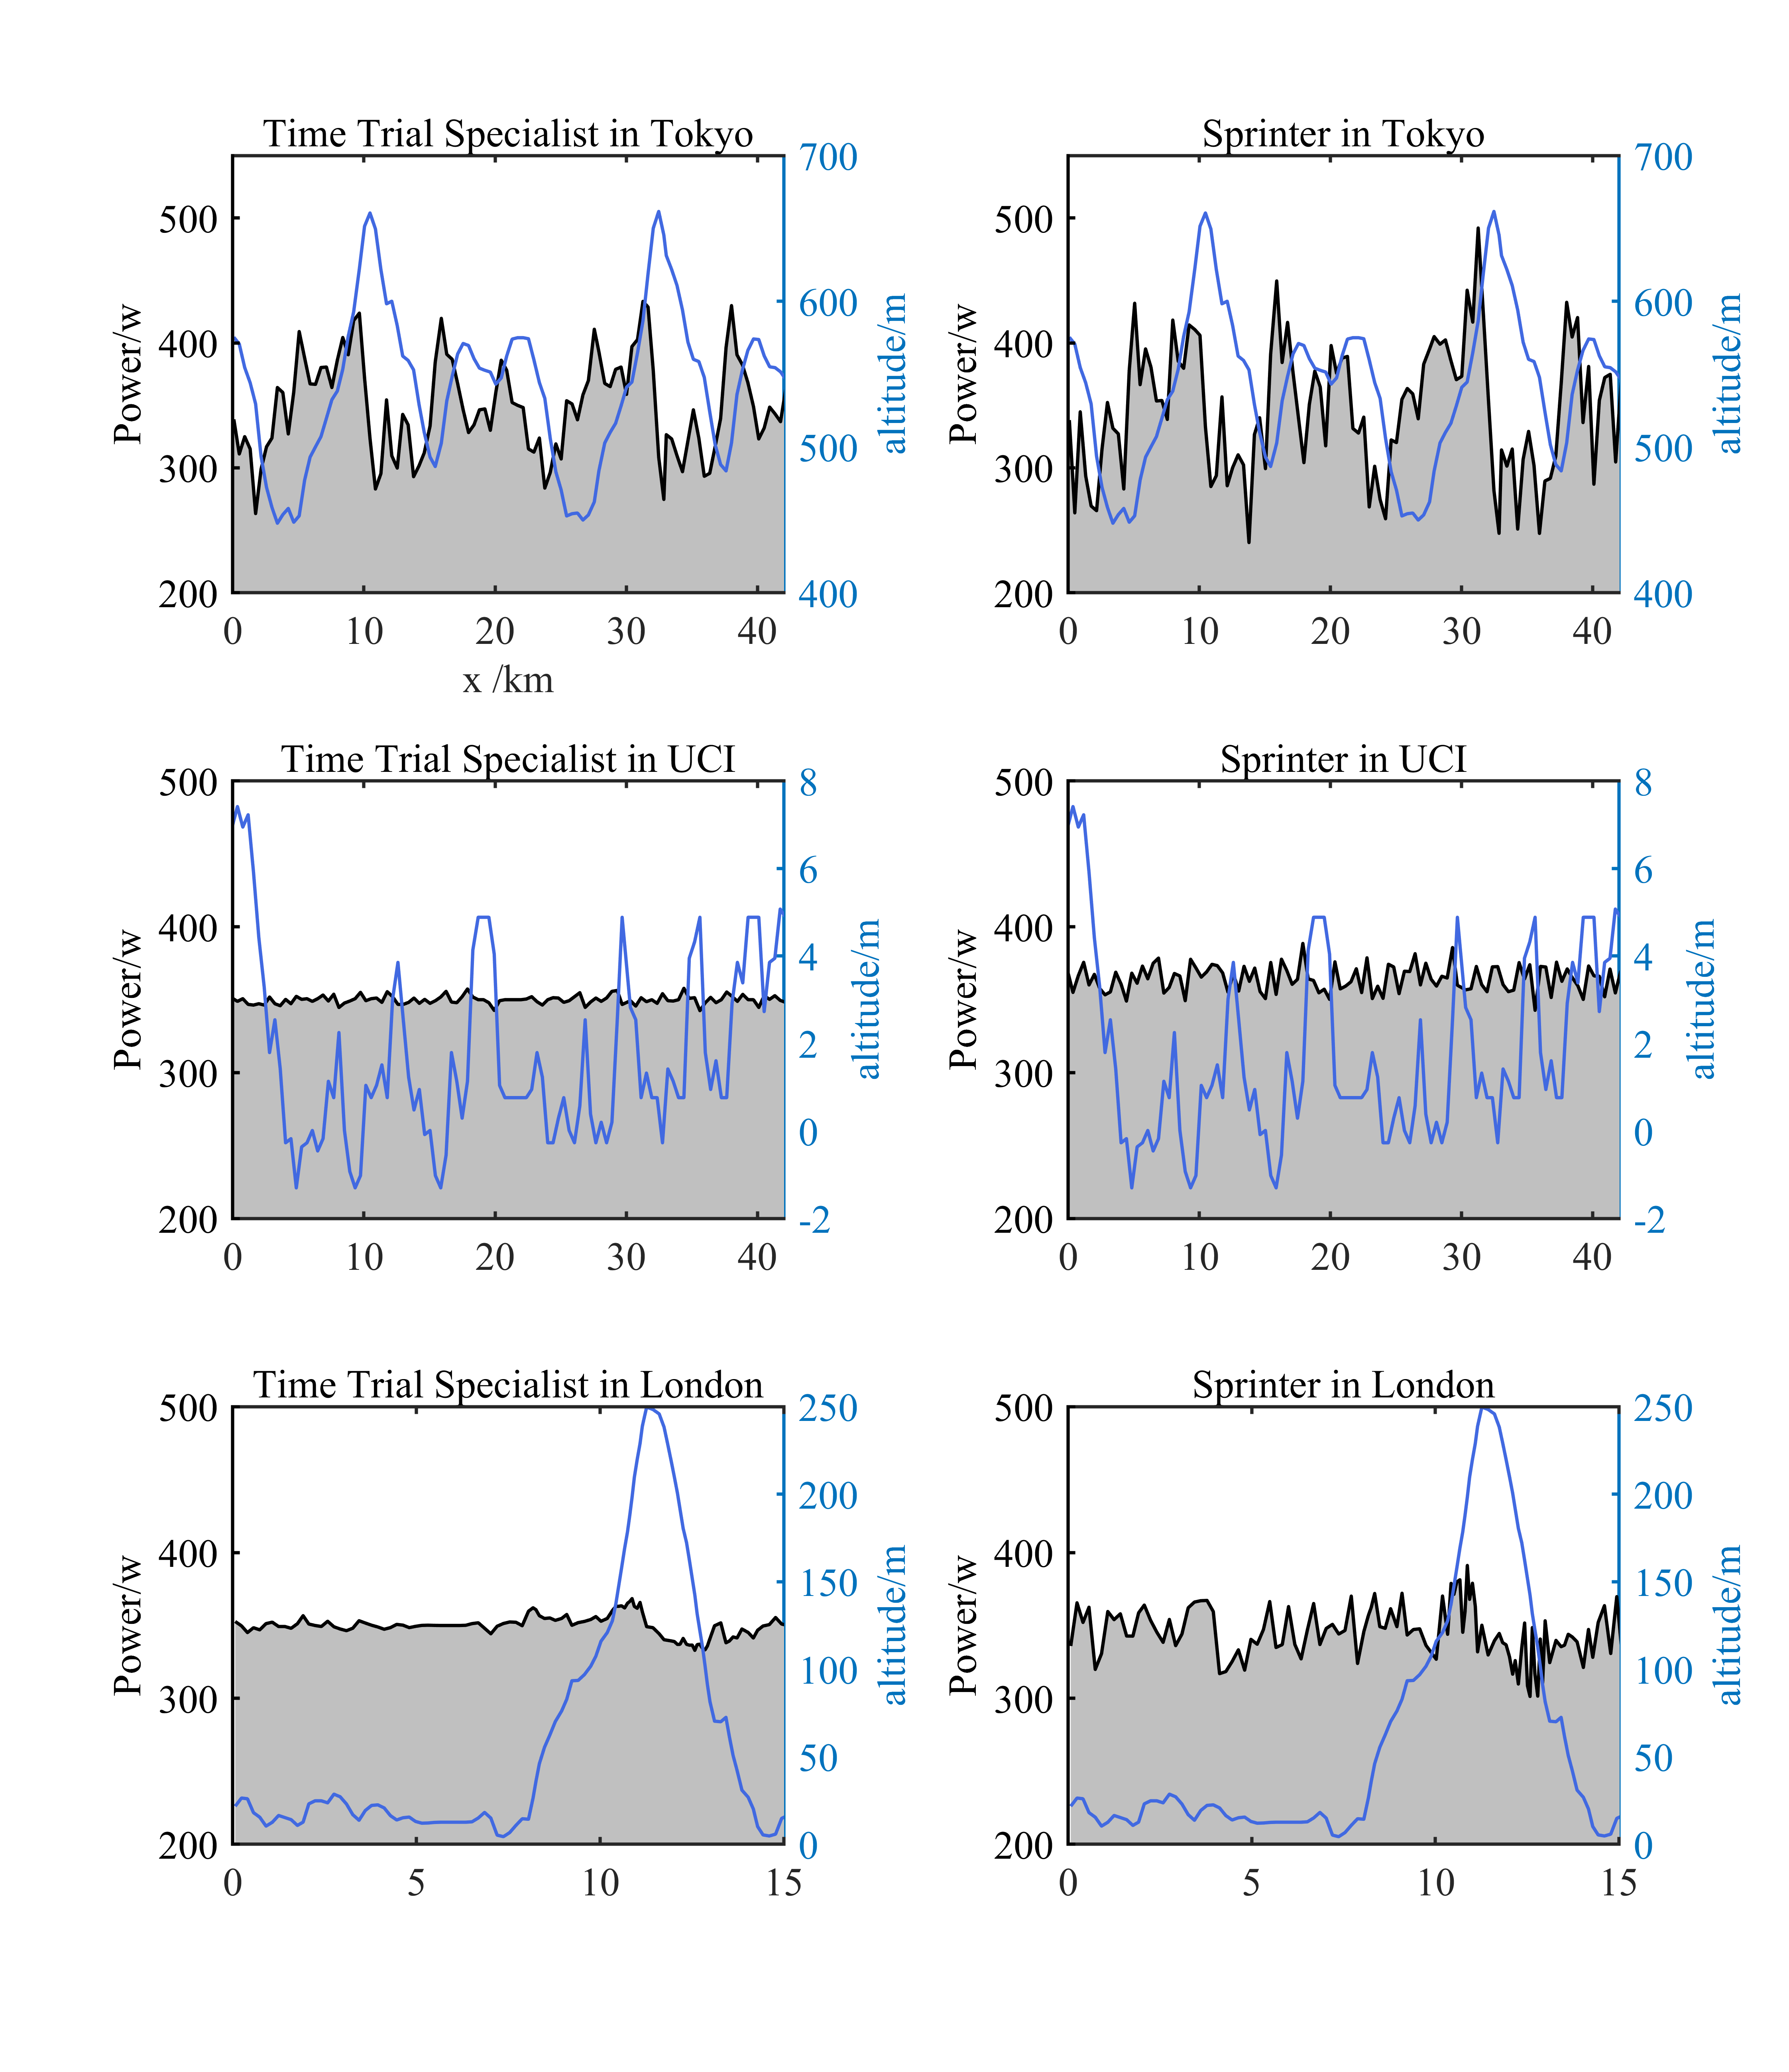
\includegraphics[width = \textwidth]{pro2}
    \caption{一个炒鸡大的插图示例}
\end{figure}
\subsection{问题二分析}
参见表1.
\begin{table}[htbp]
    % 这里默认是三线表,其他表格亲测也是可以的
    \centering
    \begin{tabular}{cccc}
        \toprule
        前缀 & 端口               & 地址范围              & 地址数量                          \\
        \midrule
        00   & 0                  & 0000 0000 - 0011 1111 & $2^6 = 64$                        \\
        010  & 1                  & 0100 0000 - 0101 1111 & $2^5 = 32$                        \\
        011  & \multirow{2}{*}{2} & 0110 0000 - 0111 1111 & \multirow{2}{*}{$2^6 + 2^5 = 96$} \\
        10   & ~                  & 1000 0000 - 1011 1111 & ~                                 \\
        11   & 3                  & 1100 0000 - 1111 1111 & $2^6 = 64$                        \\
        \bottomrule
    \end{tabular}
    \caption{一个表格示例}
\end{table}
\subsection{问题三分析}
问题三分析。
\subsection{问题四分析}
问题四分析中文文献引用\upcite{王坤峰2017生成式对抗网络}。
\section{模型假设}
这里是模型假设
\section{符号说明}
\begin{table}[H]
    \centering
    \begin{tabularx}{\textwidth}{@{}c *2{>{\centering\arraybackslash}X}@{}}
        % \begin{tabularx}{\textwidth}{ccc}
        \toprule
        符号     & 说明 & 单位 \\
        \midrule
        $\Delta$ & 0    & -    \\
        $p$      & 功率 & $W$  \\
        \bottomrule
    \end{tabularx}
    \caption{符号说明表}
\end{table}
\section{数据预处理}
我们进行了数据预处理。
\section{模型的建立与求解}
\subsection{问题一}
\subsubsection{模型的建立}
align数学环境
\begin{align}
    -r u_{i-1, j+1}+2(1+r) u_{i, j+1}-r u_{i+1, j+1}{} & {}=u_{i-1, j}+2(1-r) u_{i, j}+r u_{i+1, j} \\
    (1+\beta \triangle x) u_{1, j+1}-u_{2, j+1}{}      & {}=\beta \Delta x u_{s}(j+1)               \\
    (1+\beta \triangle x) u_{m, j+1}-u_{m-1, j+1}{}    & {}=\beta \Delta x u_{s}(j+1)
\end{align}
\subsubsection{算法描述}
算法伪代码环境
\begin{algorithm}
    \caption{算法伪代码环境}
    \label{hhsa}
    \begin{algorithmic}[]  %1表示每隔一行编号	
        \Require The original signal $x$.
        \Ensure  The energy-time-frequency distribution of $x$.
        \Function{EMD}{x, seg\_len}
        \State  N $\gets$ length(x) / seg\_len;
        \For {i=1 $\to$ i=N}
        \State seg(i) $\gets$ x(1+(i-1)*seg\_len : i*seg\_len);
        \EndFor
        \EndFunction
    \end{algorithmic}
\end{algorithm}
\subsubsection{模型的求解}
equation 等式环境测试
\begin{equation}\label{D}
    D=\sqrt{\frac{1}{N}\sum_{i=0}^N{\left| u\left( 2t^{\prime\prime}-\left( t^\prime+i\Delta t \right) \right) -u\left( t^\prime+i\Delta t \right) \right|}^2}
\end{equation}
\subsubsection{结果与分析}
这里是求解结果$q=p\times a$ 行内公式。
\subsection{问题二}
\subsubsection{模型的建立}
\subsubsection{模型的求解}
\subsection{问题三}
\subsubsection{模型的建立}
\subsubsection{模型的求解}
\section{模型评价与推广}
\subsection{模型评价}
\subsubsection{模型稳定性分析}
\begin{figure}[!htbp]
    \centering
    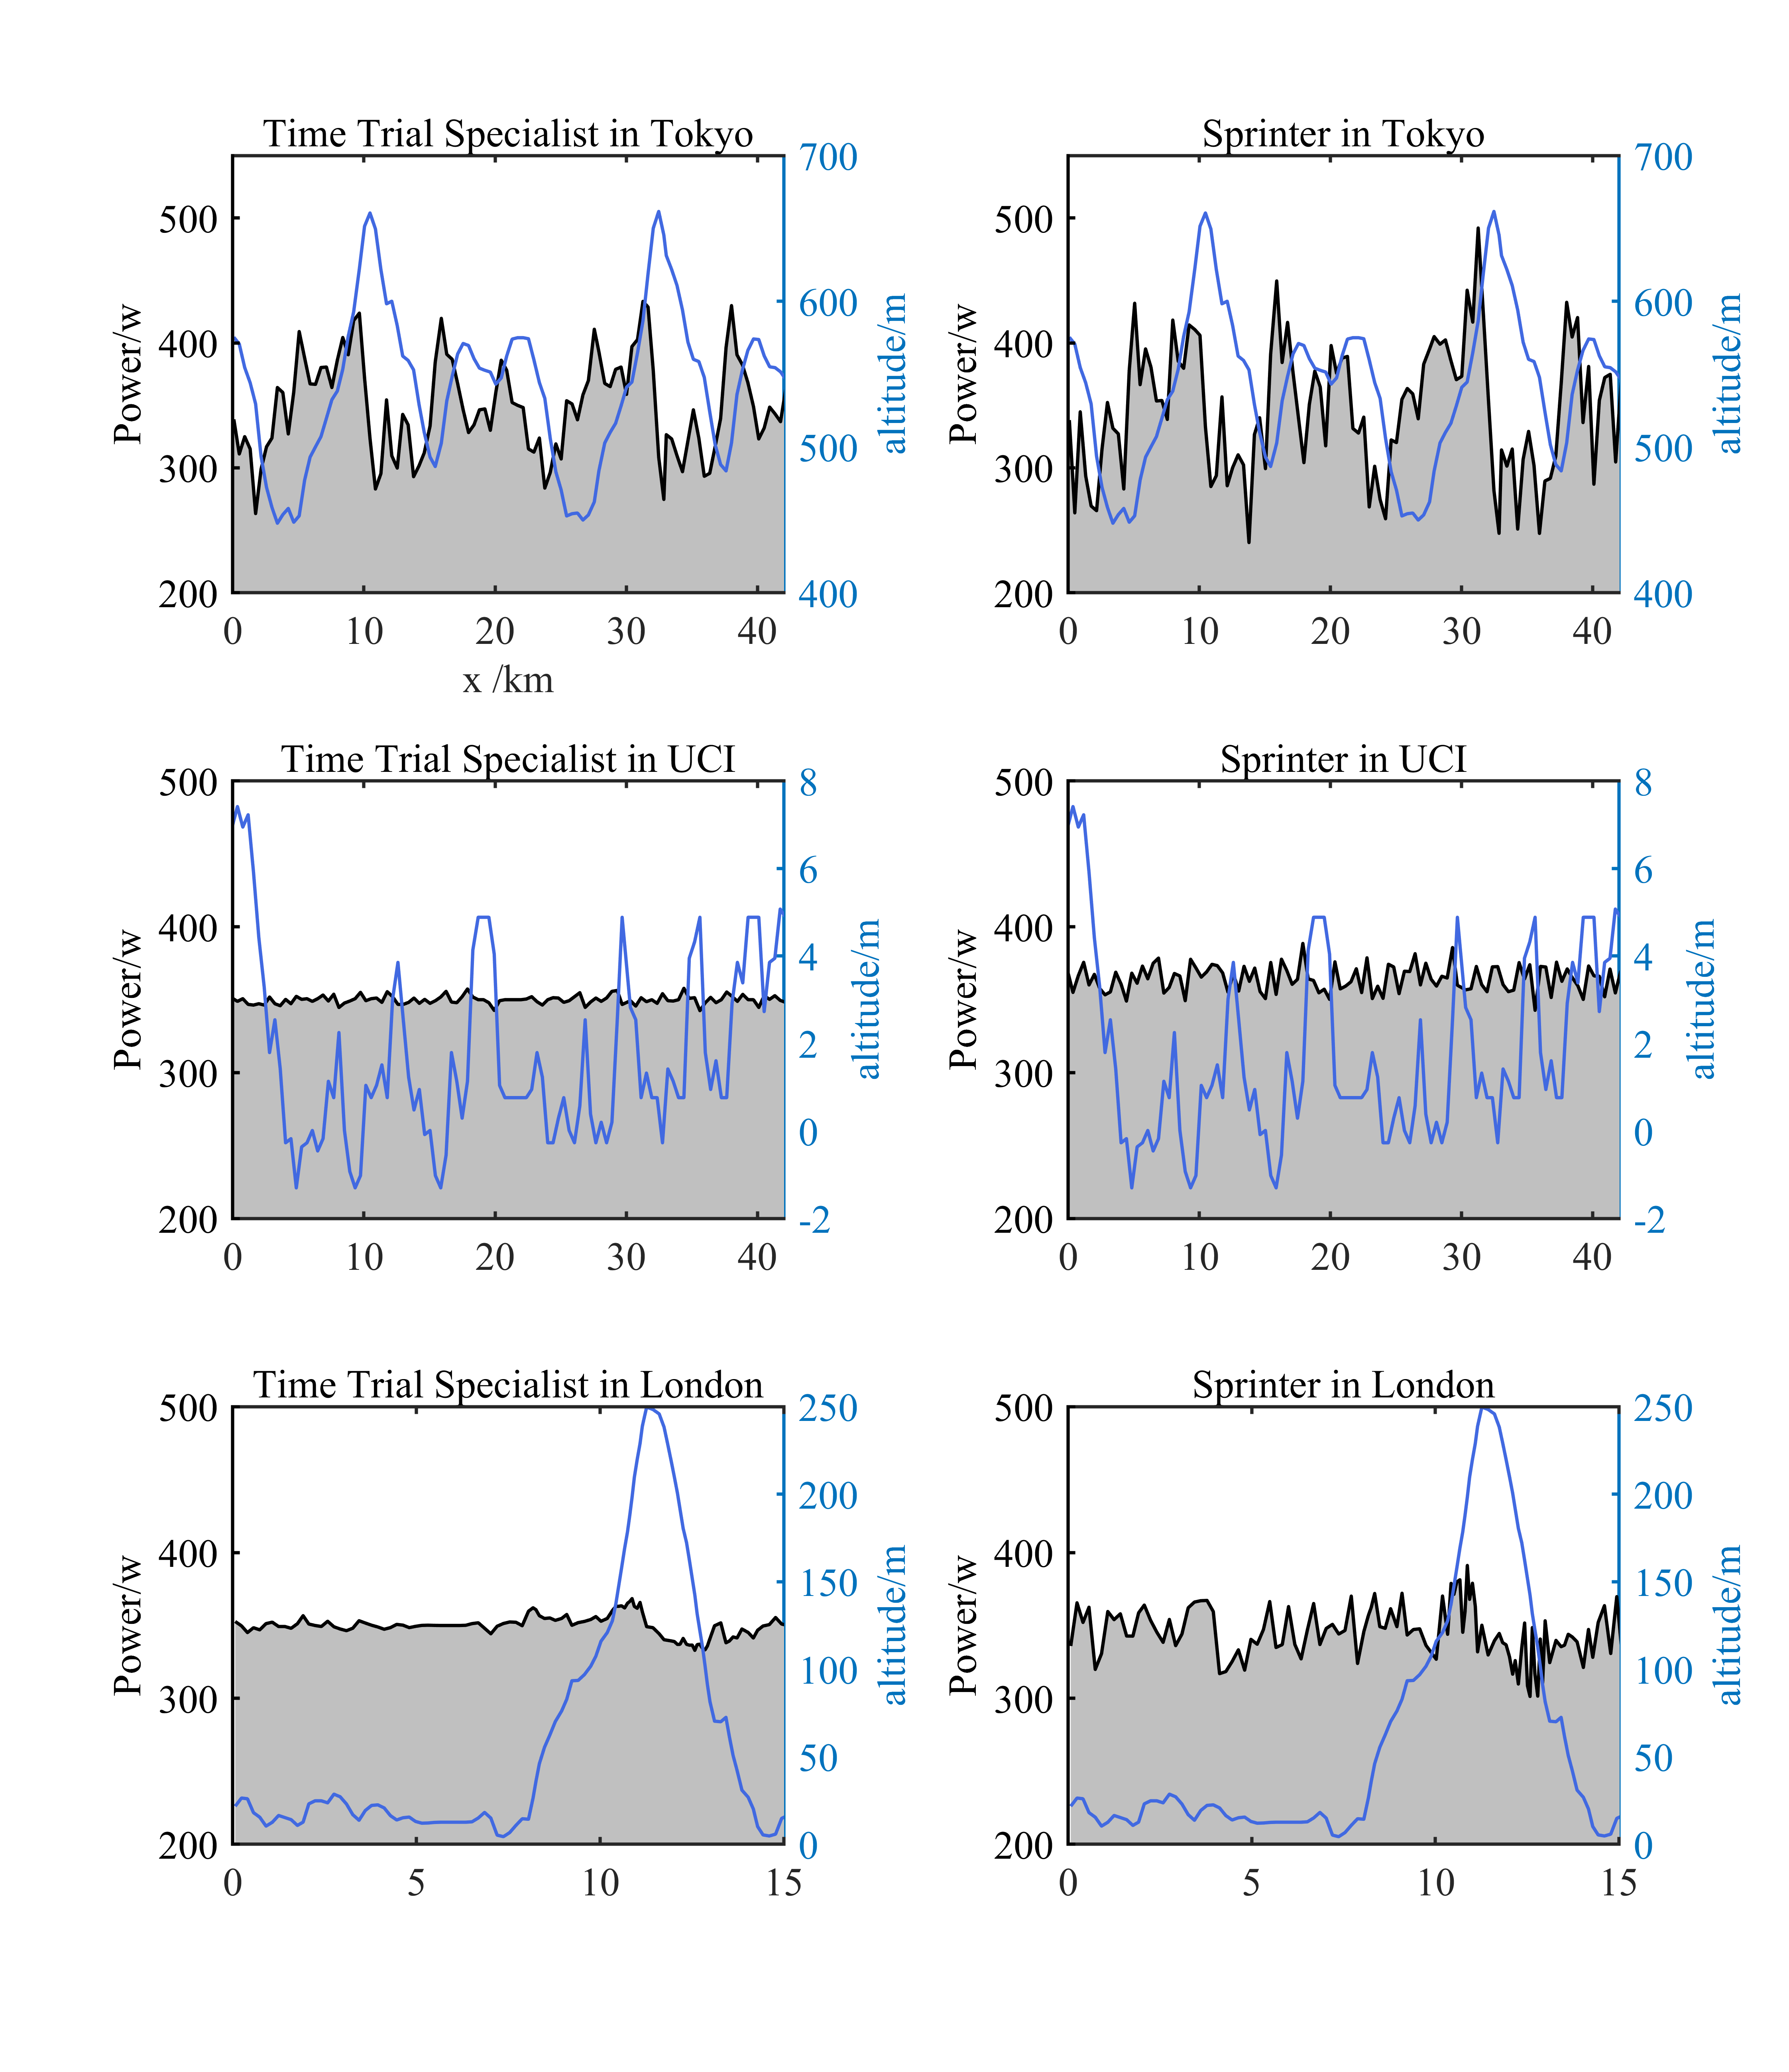
\includegraphics[width = \textwidth]{pro2}
    \caption[]{一般插图}
\end{figure}
\subsubsection{模型的优点}
\begin{itemize}
    \item 无序列表测试
    \item a
\end{itemize}
\subsection{模型的缺点}
\begin{enumerate}
    \item 有序列表测试
    \item b
\end{enumerate}
\subsection{模型推广}
一段正文一段正文一段正文一段正文一段正文一段正文一段正文一段正文一段正文一段正文一段正文一段正文一段正文一段正文一段正文一段正文一段正文一段正文一段正文一段正文一段正文一段正文一段正文一段正文一段正文一段正文一段正文一段正文一段正文一段正文一段正文一段正文一段正文一段正文一段正文一段正文一段正文一段正文一段正文一段正文一段正文一段正文一段正文一段正文一段正文一段正文一段正文一段正文一段正文一段正文一段正文一段正文一段正文一段正文一段正文一段正文一段正文一段正文一段正文一段正文一段正文一段正文一段正文一段正文一段正文一段正文一段正文一段正文一段正文一段正文一段正文一段正文一段正文一段正文一段正文。
\par 两段正文两段正文两段正文两段正文两段正文两段正文两段正文两段正文两段正文两段正文两段正文两段正文两段正文两段正文两段正文两段正文两段正文两段正文两段正文两段正文两段正文两段正文两段正文两段正文两段正文两段正文两段正文两段正文两段正文两段正文两段正文两段正文两段正文两段正文两段正文两段正文两段正文两段正文两段正文两段正文两段正文两段正文两段正文两段正文两段正文两段正文两段正文两段正文两段正文两段正文两段正文两段正文两段正文两段正文两段正文两段正文两段正文两段正文两段正文两段正文两段正文两段正文两段正文两段正文两段正文两段正文两段正文两段正文两段正文两段正文两段正文两段正文两段正文两段正文两段正文两段正文两段正文两段正文两段正文两段正文两段正文两段正文两段正文两段正文两段正文两段正文两段正文。

% 参考文献
\bibliographystyle{gbt7714-2005}
\bibliography{bib/ref.bib}

% 附录
\newpage
\begin{appendices}
    \section{代码文件列表}
    % 到时候根据文件名长度关系控制表格两栏的宽度即可
    \begin{table}[htbp]
        \centering
        \begin{tabular}{cc}
            \toprule[1.5pt]
            文件名   & 功能描述 \\
            \midrule
            Data.mat & 附件数据 \\
            \bottomrule
        \end{tabular}
    \end{table}

    % 附件:在论文附录部分插入所用到的所有代码和命令交互序列
    \section{代码}
    problem1.py 用来处理$\cdots$逻辑。
    \par \lstinputlisting[language=python]{code/problem1.py}
    \par problem1.m用于处理$\cdots$逻辑。
    \par \lstinputlisting[language = matlab]{code/problem1.m}
\end{appendices}

\end{document}